\documentclass{beamer}
\usetheme{metropolis}
\usepackage{graphicx}
\usepackage{amsmath}
\usepackage{tcolorbox}

\def\rcurs{{\mbox{$\resizebox{.16in}{.08in}{
\includegraphics{ScriptR}}$}}}
\def\brcurs{{\mbox{$\resizebox{.16in}{.08in}{
\includegraphics{BoldR}}$}}}
\def\hrcurs{{\mbox{$\hat \brcurs$}}}

\title{Electromagnetc Theory: PHYS330}
\author{Jordan Hanson}
\institute{Whittier College Department of Physics and Astronomy}

\begin{document}
\maketitle

\section{Summary}

\begin{frame}{Week 3 Summary}
\begin{enumerate}
\item Laplace's Equation
\begin{itemize}
\item One-dimension
\item Two-dimensions, three dimensions, uniqueness, boundaries
\end{itemize}
\item Separation of Variables: Boundary-value problems
\begin{itemize}
\item Cartesian coordinates
\item Spherical coordinates
\end{itemize}
\item Multipole Expansions
\begin{itemize}
\item Far-fields
\item Monopole and dipole terms
\item Electric Field of a Dipole
\end{itemize}
\end{enumerate}
\end{frame}

\section{Laplace's Equation: One Dimension}

\begin{frame}{Laplace's Equation: One dimension}
\alert{\textbf{Laplace's Equation in one dimension:}}
\begin{equation}
\frac{d^2V}{dx^2} = 0
\end{equation}
What is the solution?
\begin{equation}
V(x) = mx + b
\end{equation}
What is the magnitude of the E-field?
\begin{itemize}
\item A: $V(x)$
\item B: $x$
\item C: $b$
\item D: $m$
\end{itemize}
\end{frame}

\begin{frame}{Laplace's Equation: One dimension}
\begin{figure}
\centering
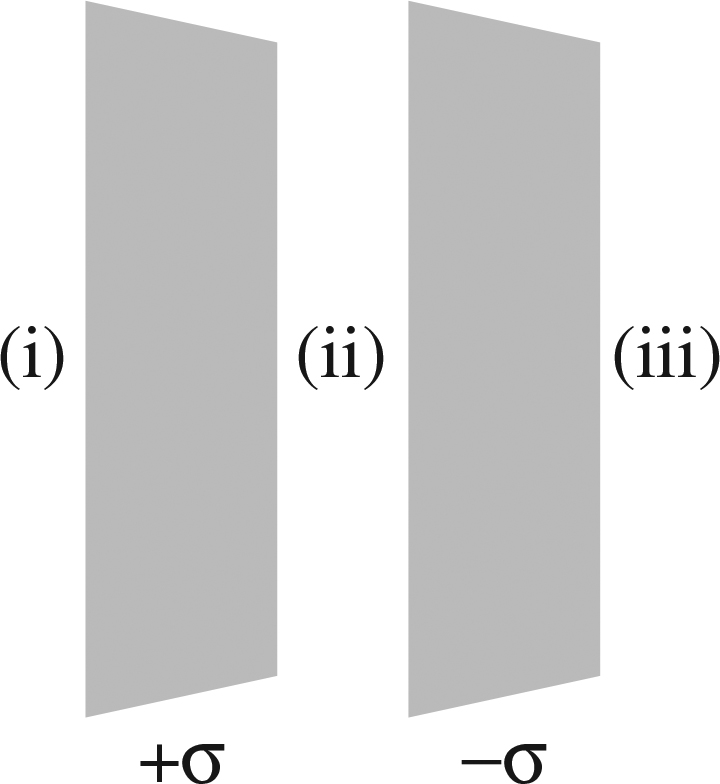
\includegraphics[width=6cm]{figures/2_23.jpg}
\caption{\label{fig:cap} The setup of a parallel plate capacitor.}
\end{figure}
\end{frame}

\begin{frame}{Laplace's Equation: One dimension}
\small
Suppose the negative side of the parallel plate capacitor is grounded, and the positive side is at a potential $V_0$.  Let the separation between the plates be $x_0$.  Further, let the positive plate occupy the yz plane, passing through the origin.  Find the E-field magnitude and direction by solving Laplace's equation. \\ \vspace{6cm}
\end{frame}

\begin{frame}{Laplace's Equation: One dimension}
\small
Show that the potential of a point charge at the origin satisfies Laplace's Equation for $r\neq 0$.  \textit{Use the form of the Laplacian in spherical coordinates.}\\ \vspace{6cm}
\end{frame}

\section{Conclusion}

\begin{frame}{Week 3 Summary}
\begin{enumerate}
\item Laplace's Equation
\begin{itemize}
\item One-dimension
\item Two-dimensions, three dimensions, uniqueness, boundaries
\end{itemize}
\item Separation of Variables: Boundary-value problems
\begin{itemize}
\item Cartesian coordinates
\item Spherical coordinates
\end{itemize}
\item Multipole Expansions
\begin{itemize}
\item Far-fields
\item Monopole and dipole terms
\item Electric Field of a Dipole
\end{itemize}
\end{enumerate}
\end{frame}

\end{document}
